% Options for packages loaded elsewhere
\PassOptionsToPackage{unicode}{hyperref}
\PassOptionsToPackage{hyphens}{url}
%
\documentclass[
]{article}
\usepackage{amsmath,amssymb}
\usepackage{lmodern}
\usepackage{iftex}
\ifPDFTeX
  \usepackage[T1]{fontenc}
  \usepackage[utf8]{inputenc}
  \usepackage{textcomp} % provide euro and other symbols
\else % if luatex or xetex
  \usepackage{unicode-math}
  \defaultfontfeatures{Scale=MatchLowercase}
  \defaultfontfeatures[\rmfamily]{Ligatures=TeX,Scale=1}
\fi
% Use upquote if available, for straight quotes in verbatim environments
\IfFileExists{upquote.sty}{\usepackage{upquote}}{}
\IfFileExists{microtype.sty}{% use microtype if available
  \usepackage[]{microtype}
  \UseMicrotypeSet[protrusion]{basicmath} % disable protrusion for tt fonts
}{}
\makeatletter
\@ifundefined{KOMAClassName}{% if non-KOMA class
  \IfFileExists{parskip.sty}{%
    \usepackage{parskip}
  }{% else
    \setlength{\parindent}{0pt}
    \setlength{\parskip}{6pt plus 2pt minus 1pt}}
}{% if KOMA class
  \KOMAoptions{parskip=half}}
\makeatother
\usepackage{xcolor}
\IfFileExists{xurl.sty}{\usepackage{xurl}}{} % add URL line breaks if available
\IfFileExists{bookmark.sty}{\usepackage{bookmark}}{\usepackage{hyperref}}
\hypersetup{
  pdftitle={Untitled},
  hidelinks,
  pdfcreator={LaTeX via pandoc}}
\urlstyle{same} % disable monospaced font for URLs
\usepackage[margin=1in]{geometry}
\usepackage{color}
\usepackage{fancyvrb}
\newcommand{\VerbBar}{|}
\newcommand{\VERB}{\Verb[commandchars=\\\{\}]}
\DefineVerbatimEnvironment{Highlighting}{Verbatim}{commandchars=\\\{\}}
% Add ',fontsize=\small' for more characters per line
\usepackage{framed}
\definecolor{shadecolor}{RGB}{248,248,248}
\newenvironment{Shaded}{\begin{snugshade}}{\end{snugshade}}
\newcommand{\AlertTok}[1]{\textcolor[rgb]{0.94,0.16,0.16}{#1}}
\newcommand{\AnnotationTok}[1]{\textcolor[rgb]{0.56,0.35,0.01}{\textbf{\textit{#1}}}}
\newcommand{\AttributeTok}[1]{\textcolor[rgb]{0.77,0.63,0.00}{#1}}
\newcommand{\BaseNTok}[1]{\textcolor[rgb]{0.00,0.00,0.81}{#1}}
\newcommand{\BuiltInTok}[1]{#1}
\newcommand{\CharTok}[1]{\textcolor[rgb]{0.31,0.60,0.02}{#1}}
\newcommand{\CommentTok}[1]{\textcolor[rgb]{0.56,0.35,0.01}{\textit{#1}}}
\newcommand{\CommentVarTok}[1]{\textcolor[rgb]{0.56,0.35,0.01}{\textbf{\textit{#1}}}}
\newcommand{\ConstantTok}[1]{\textcolor[rgb]{0.00,0.00,0.00}{#1}}
\newcommand{\ControlFlowTok}[1]{\textcolor[rgb]{0.13,0.29,0.53}{\textbf{#1}}}
\newcommand{\DataTypeTok}[1]{\textcolor[rgb]{0.13,0.29,0.53}{#1}}
\newcommand{\DecValTok}[1]{\textcolor[rgb]{0.00,0.00,0.81}{#1}}
\newcommand{\DocumentationTok}[1]{\textcolor[rgb]{0.56,0.35,0.01}{\textbf{\textit{#1}}}}
\newcommand{\ErrorTok}[1]{\textcolor[rgb]{0.64,0.00,0.00}{\textbf{#1}}}
\newcommand{\ExtensionTok}[1]{#1}
\newcommand{\FloatTok}[1]{\textcolor[rgb]{0.00,0.00,0.81}{#1}}
\newcommand{\FunctionTok}[1]{\textcolor[rgb]{0.00,0.00,0.00}{#1}}
\newcommand{\ImportTok}[1]{#1}
\newcommand{\InformationTok}[1]{\textcolor[rgb]{0.56,0.35,0.01}{\textbf{\textit{#1}}}}
\newcommand{\KeywordTok}[1]{\textcolor[rgb]{0.13,0.29,0.53}{\textbf{#1}}}
\newcommand{\NormalTok}[1]{#1}
\newcommand{\OperatorTok}[1]{\textcolor[rgb]{0.81,0.36,0.00}{\textbf{#1}}}
\newcommand{\OtherTok}[1]{\textcolor[rgb]{0.56,0.35,0.01}{#1}}
\newcommand{\PreprocessorTok}[1]{\textcolor[rgb]{0.56,0.35,0.01}{\textit{#1}}}
\newcommand{\RegionMarkerTok}[1]{#1}
\newcommand{\SpecialCharTok}[1]{\textcolor[rgb]{0.00,0.00,0.00}{#1}}
\newcommand{\SpecialStringTok}[1]{\textcolor[rgb]{0.31,0.60,0.02}{#1}}
\newcommand{\StringTok}[1]{\textcolor[rgb]{0.31,0.60,0.02}{#1}}
\newcommand{\VariableTok}[1]{\textcolor[rgb]{0.00,0.00,0.00}{#1}}
\newcommand{\VerbatimStringTok}[1]{\textcolor[rgb]{0.31,0.60,0.02}{#1}}
\newcommand{\WarningTok}[1]{\textcolor[rgb]{0.56,0.35,0.01}{\textbf{\textit{#1}}}}
\usepackage{longtable,booktabs,array}
\usepackage{calc} % for calculating minipage widths
% Correct order of tables after \paragraph or \subparagraph
\usepackage{etoolbox}
\makeatletter
\patchcmd\longtable{\par}{\if@noskipsec\mbox{}\fi\par}{}{}
\makeatother
% Allow footnotes in longtable head/foot
\IfFileExists{footnotehyper.sty}{\usepackage{footnotehyper}}{\usepackage{footnote}}
\makesavenoteenv{longtable}
\usepackage{graphicx}
\makeatletter
\def\maxwidth{\ifdim\Gin@nat@width>\linewidth\linewidth\else\Gin@nat@width\fi}
\def\maxheight{\ifdim\Gin@nat@height>\textheight\textheight\else\Gin@nat@height\fi}
\makeatother
% Scale images if necessary, so that they will not overflow the page
% margins by default, and it is still possible to overwrite the defaults
% using explicit options in \includegraphics[width, height, ...]{}
\setkeys{Gin}{width=\maxwidth,height=\maxheight,keepaspectratio}
% Set default figure placement to htbp
\makeatletter
\def\fps@figure{htbp}
\makeatother
\setlength{\emergencystretch}{3em} % prevent overfull lines
\providecommand{\tightlist}{%
  \setlength{\itemsep}{0pt}\setlength{\parskip}{0pt}}
\setcounter{secnumdepth}{5}
\usepackage{subfig}
\ifLuaTeX
  \usepackage{selnolig}  % disable illegal ligatures
\fi

\title{Untitled}
\author{}
\date{\vspace{-2.5em}2022-06-11}

\begin{document}
\maketitle

{
\setcounter{tocdepth}{2}
\tableofcontents
}
\hypertarget{r-markdown}{%
\subsection{R Markdown}\label{r-markdown}}

\begin{Shaded}
\begin{Highlighting}[]
\NormalTok{EViews\textgreater{} wfcreate(wf=sagiru,page=mati) q 2000 2025}
\NormalTok{+ for \%y page1 page2 page3 page4}
\NormalTok{+ pagecreate(page=\{\%y\}) q 2000 2025}
\NormalTok{+ next}
\NormalTok{+ \%pagelist=@pagelist}
\NormalTok{+ \textquotesingle{}open mychunk}
\NormalTok{+ for \%y \{\%pagelist\}}
\NormalTok{+ pageselect \{\%y\}}
\NormalTok{+ delete gra*}
\NormalTok{+ genr y=@cumsum(nrnd)}
\NormalTok{+ genr x=@cumsum(nrnd)}
\NormalTok{+ genr z=@cumsum(nrnd)}
\NormalTok{+ genr date=@date}
\NormalTok{+                      graph grap1.line z  }
\NormalTok{+                            graph grap2.line z y x}
\NormalTok{+    freeze(grap,mode=overwrite) x.line}
\NormalTok{+ equation ols.ls y c x}
\NormalTok{+ freeze(tab) ols}
\NormalTok{+ next}
\NormalTok{+ wfsave mychunk}
\end{Highlighting}
\end{Shaded}

\begin{verbatim}
##        aic  df     coefs       dw        f    fprob       hq      logl  meandep
## 1 5.917171 102 -3.513948 0.078297 102.2672 4.58e-17 5.937773 -305.6929 4.854126
## 2       NA  NA  0.851298       NA       NA       NA       NA        NA       NA
##   ncoef     pval       r2    rbar2 regobs  schwarz    sddep       se      ssr
## 1     2 3.20e-04 0.500654 0.495759    104 5.968024 6.504375 4.618754 2175.955
## 2    NA 4.58e-17       NA       NA     NA       NA       NA       NA       NA
##    stderrs    tstats
## 1 0.943317 -3.725099
## 2 0.084181 10.112730
\end{verbatim}

\begin{verbatim}
##        aic  df     coefs       dw        f    fprob       hq      logl  meandep
## 1 5.917171 102 -3.513948 0.078297 102.2672 4.58e-17 5.937773 -305.6929 4.854126
## 2       NA  NA  0.851298       NA       NA       NA       NA        NA       NA
##   ncoef     pval       r2    rbar2 regobs  schwarz    sddep       se      ssr
## 1     2 3.20e-04 0.500654 0.495759    104 5.968024 6.504375 4.618754 2175.955
## 2    NA 4.58e-17       NA       NA     NA       NA       NA       NA       NA
##    stderrs    tstats
## 1 0.943317 -3.725099
## 2 0.084181 10.112730
\end{verbatim}

\begin{verbatim}
##           Dependent.Variable..Y           X                       X.1
## 1         Method: Least Squares                                      
## 2  Date: 06/21/22   Time: 08:19                                      
## 3         Sample: 2000Q1 2025Q4                                      
## 4    Included observations: 104                                      
## 5                                                                    
## 6                      Variable Coefficient                Std. Error
## 7                                                                    
## 8                             C   -3.513948                  0.943317
## 9                             X    0.851298                  0.084181
## 10                                                                   
## 11                    R-squared    0.500654        Mean dependent var
## 12           Adjusted R-squared    0.495759        S.D. dependent var
## 13           S.E. of regression    4.618754     Akaike info criterion
## 14            Sum squared resid    2175.955         Schwarz criterion
## 15               Log likelihood   -305.6929      Hannan-Quinn criter.
## 16                  F-statistic    102.2672        Durbin-Watson stat
## 17            Prob(F-statistic)    0.000000                          
## 18                                                                   
##            X.2      X.3
## 1                      
## 2                      
## 3                      
## 4                      
## 5                      
## 6  t-Statistic  Prob.  
## 7                      
## 8    -3.725099   0.0003
## 9     10.11273   0.0000
## 10                     
## 11             4.854126
## 12             6.504375
## 13             5.917171
## 14             5.968024
## 15             5.937773
## 16             0.078297
## 17                     
## 18
\end{verbatim}

\begin{verbatim}
##         date          x           y          z
## 1 2000-01-01 -0.1764268  0.82553279 -0.8597092
## 2 2000-04-01 -0.8585432  0.47004426 -1.4952354
## 3 2000-07-01 -1.4277713  0.72106428 -2.0666701
## 4 2000-10-01 -1.5665197 -0.83778156 -3.2763182
## 5 2001-01-01 -2.0204583 -0.09023613 -5.2876991
## 6 2001-04-01 -1.3490041 -0.10562838 -6.3244963
\end{verbatim}

\hypertarget{r-plots}{%
\section{R plots}\label{r-plots}}

\begin{verbatim}
## NULL
\end{verbatim}

\begin{verbatim}
## [1] "asis"
\end{verbatim}

\begin{figure}[h]

{\centering 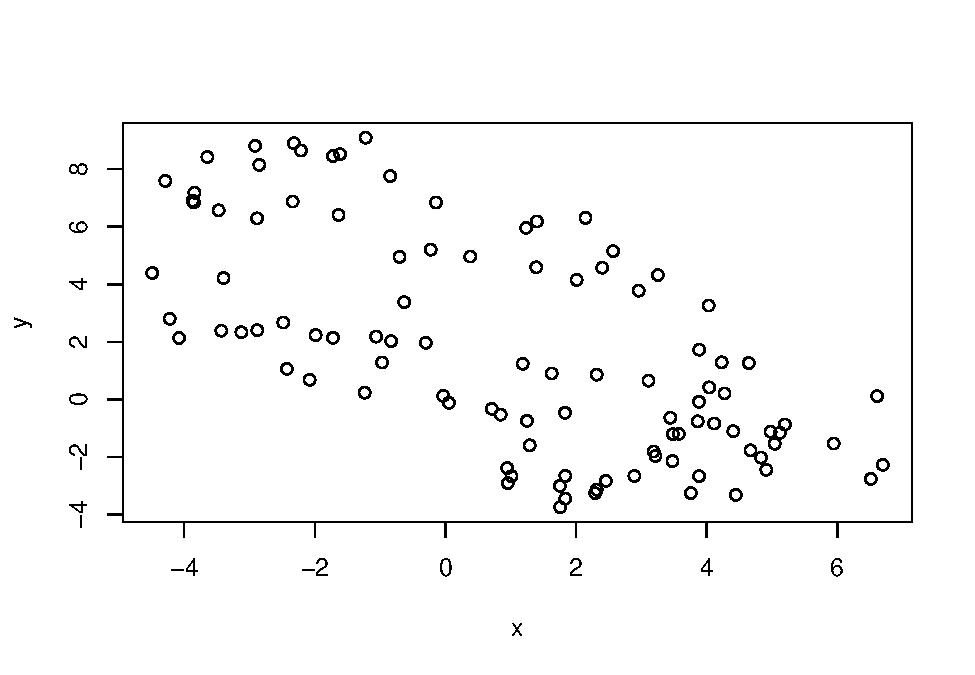
\includegraphics[width=\textwidth]{test_engEviews_files/figure-latex/labe-1} 

}

\caption{another fig}\label{fig:labe}
\end{figure}

\begin{center}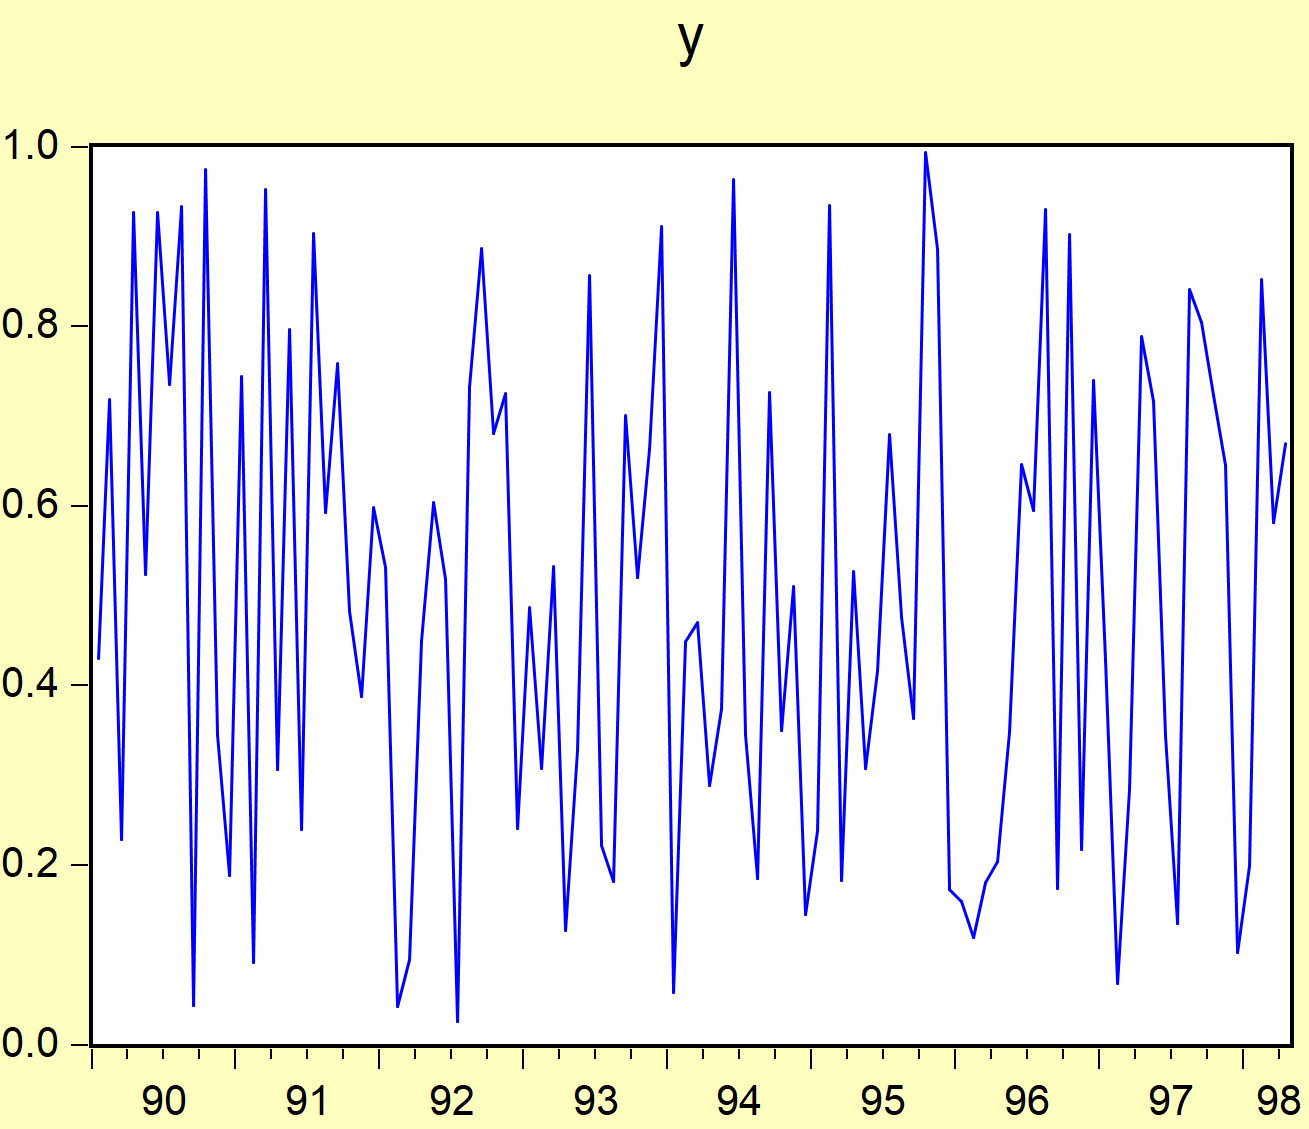
\includegraphics[width=\textwidth]{test_engEviews_files/figure-latex//eview-graph-y} \end{center}

\begin{center}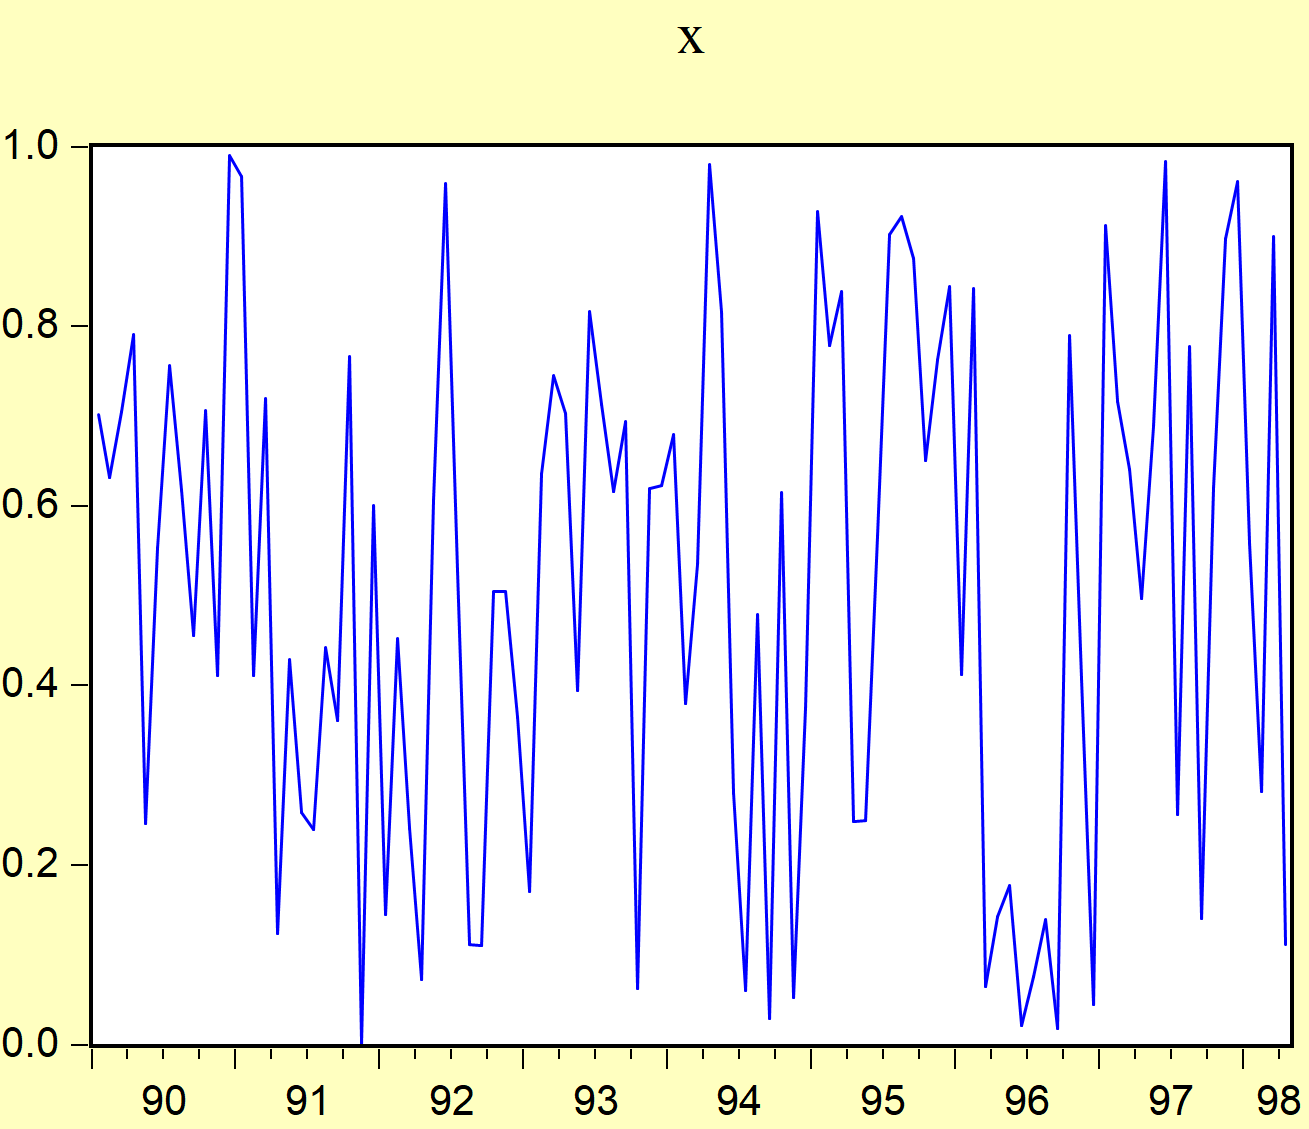
\includegraphics[width=\textwidth]{test_engEviews_files/figure-latex//eview-graph-x} \end{center}

\begin{verbatim}
##         date           x            y         z
## 1 2001-01-01  0.96611785  0.722339900 -2.279482
## 2 2001-01-02 -0.24151933  0.883142132 -1.464104
## 3 2001-01-03 -0.02438748 -0.004796057 -1.833490
## 4 2001-01-04  1.06441681  0.381263203 -1.460074
## 5 2001-01-05  0.04504655  0.525364741 -1.130334
## 6 2001-01-06 -0.01245917  0.987442426 -1.423734
\end{verbatim}

\begin{center}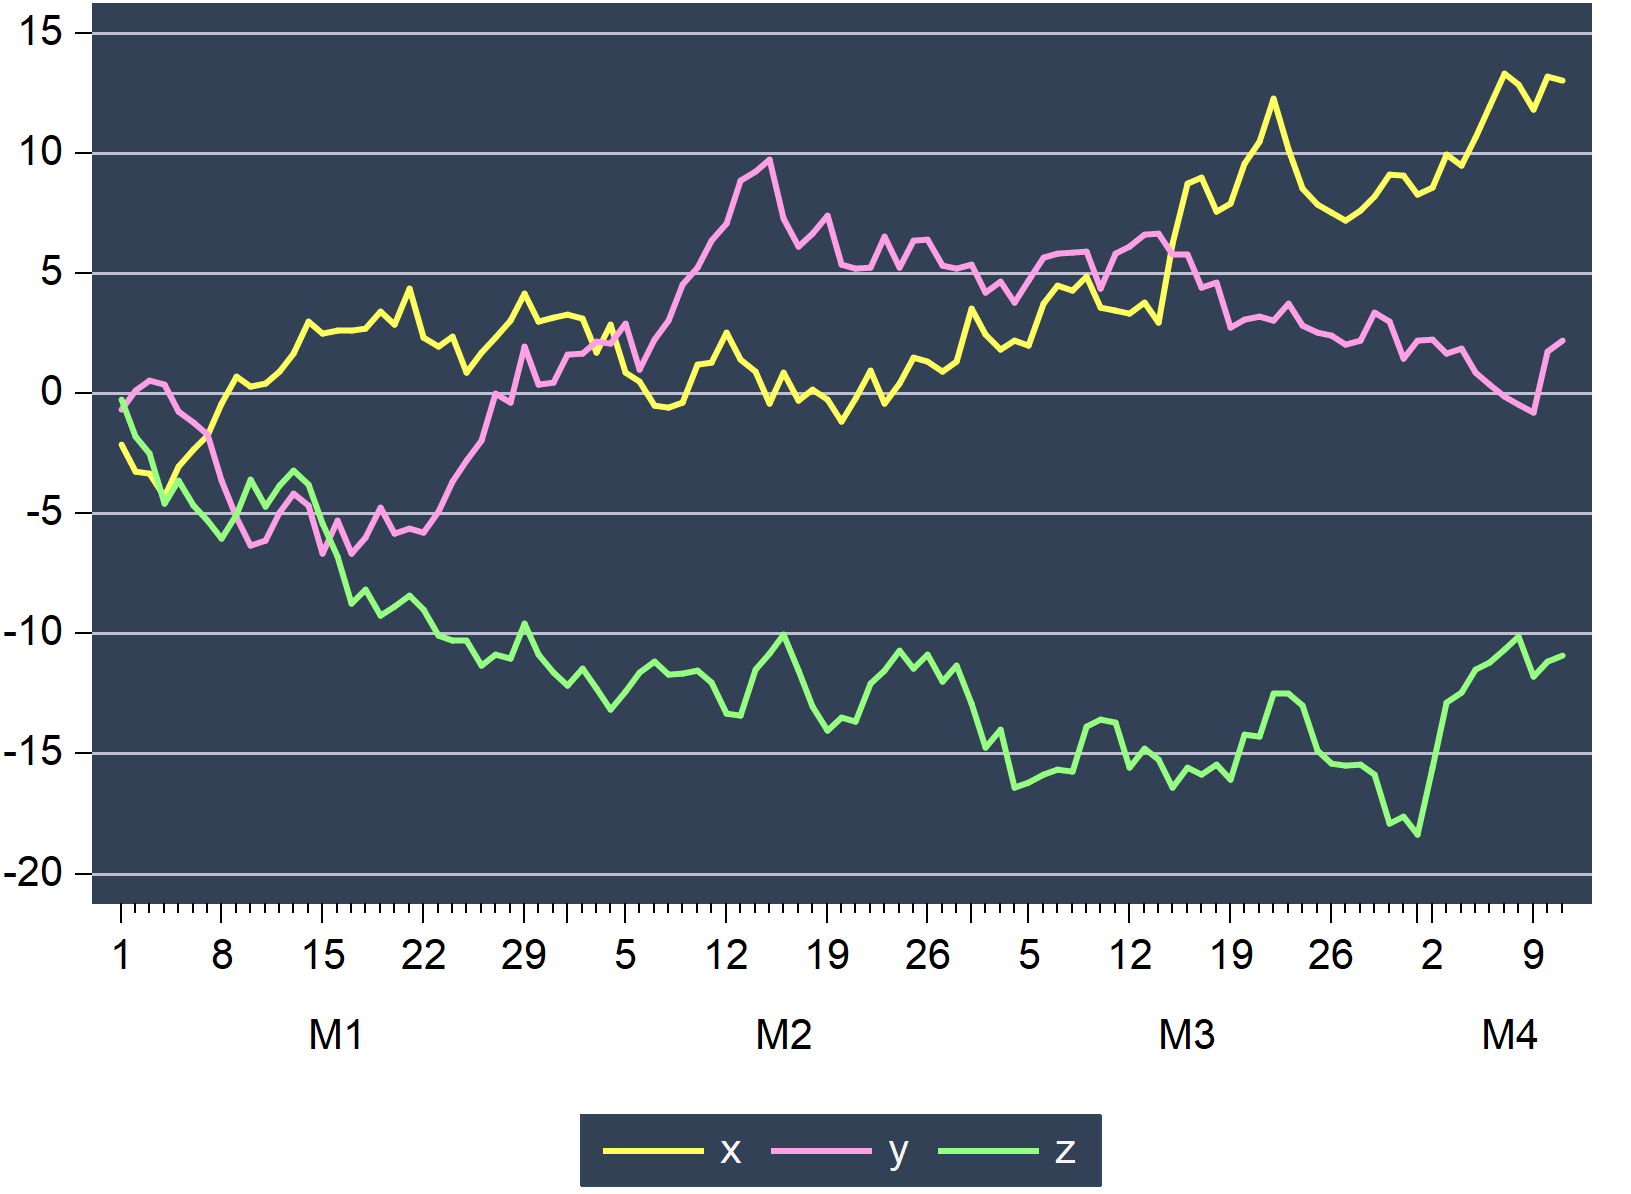
\includegraphics[width=\textwidth]{test_engEviews_files/figure-latex//rwalk-xyz} \end{center}

\end{document}
